\documentclass[hyperref={bookmarks=false},aspectratio=169]{beamer}
\usepackage{hyperref,ragged2e,amsmath,amssymb,url,bm}
\usepackage{graphicx,booktabs,array}
\usepackage{tikz}
\usetikzlibrary{arrows.meta,positioning,calc,shapes.geometric,decorations.pathreplacing,matrix}
\graphicspath{{crops/}}
\usetheme{Goettingen}
% --- Paleta de la serie Festividades santas: tierra roja, café rojizo, mostaza y papiro ---
\definecolor{tierraroja}{RGB}{122,40,18}
\definecolor{caferojizo}{RGB}{58,18,8}
\definecolor{mostaza}{RGB}{214,160,58}
\definecolor{papiro}{RGB}{243,228,192}
\definecolor{sepia}{RGB}{98,66,44}
\definecolor{oliva}{RGB}{92,98,48}
\setbeamercolor{structure}{fg=tierraroja}
\setbeamertemplate{sidebar canvas right}[vertical shading][top=tierraroja!92!black,bottom=caferojizo]
\setbeamercolor{title in sidebar}{fg=mostaza}
\setbeamercolor{author in sidebar}{fg=papiro}
\setbeamercolor{section in sidebar}{fg=papiro}
\setbeamercolor{section in sidebar shaded}{fg=mostaza!55!papiro!75!tierraroja}
\setbeamercolor{subsection in sidebar}{fg=papiro}
\setbeamercolor{subsection in sidebar shaded}{fg=mostaza!55!papiro!75!tierraroja}
\let\raggedright\justifying
\setlength{\RaggedRightRightskip}{0pt plus 1fil}
\setbeamertemplate{background canvas}{
\includegraphics[width=\paperwidth,height=\paperheight]{papiro.jpg}}
\setbeamercolor{normal text}{fg=caferojizo!90!black}
\setbeamercolor{frametitle}{fg=tierraroja}
\setbeamerfont{frametitle}{series=\bfseries}
\setbeamertemplate{section in toc shaded}{\leavevmode{\color{sepia!85!black}\inserttocsection}\par}
\setbeamercolor{title}{fg=tierraroja}
\setbeamercolor{subtitle}{fg=sepia}
\setbeamercolor{item projected}{bg=tierraroja,fg=papiro}
\setbeamertemplate{itemize item}{\small\textcolor{mostaza!80!tierraroja}{$\blacktriangleright$}}
\setbeamertemplate{navigation symbols}{}
% --- Español + hebreo + griego (XeLaTeX) con fuentes empaquetadas en fonts/ ---
\usepackage[bidi=default]{babel}
\babelprovide[import,main]{spanish}
\babelprovide[import]{hebrew}
\babelprovide[import]{ancientgreek}
\babelfont[hebrew]{sf}[Path=fonts/, BoldFont=NotoHebrewSans-700.ttf]{NotoHebrewSans-400.ttf}
\babelfont[hebrew]{rm}[Path=fonts/, BoldFont=NotoHebrewSans-700.ttf]{NotoHebrewSans-400.ttf}
\babelfont[ancientgreek]{sf}[Path=fonts/]{GFSPorson.otf}
\babelfont[ancientgreek]{rm}[Path=fonts/]{GFSPorson.otf}
\newcommand{\heb}[1]{\mbox{\foreignlanguage{hebrew}{#1}}}
\newcommand{\grc}[1]{\foreignlanguage{ancientgreek}{#1}}
\newcommand{\SENOR}{S{\fontsize{0.78em}{1em}\selectfont EÑOR}}
% --- Citas, imágenes, referencias ---
\usepackage[most]{tcolorbox}
\newtcolorbox{cita}[1][]{enhanced, colback=papiro, opacityback=0.80, colframe=tierraroja!85!mostaza,
  boxrule=0pt, leftrule=2.5pt, arc=0pt, left=6pt, right=6pt, top=4pt, bottom=4pt,
  before skip=4pt, after skip=6pt, fontupper=\small\itshape, #1}
\newcommand{\fuente}[1]{\par\hfill{\upshape\bfseries\footnotesize\textcolor{tierraroja}{#1}}}
\newcommand{\imagen}[3][0.80]{%
  \centering\includegraphics[height=#1\textheight,width=\linewidth,keepaspectratio]{#2}\par\vspace{2pt}
  {\fontsize{5}{6}\selectfont\color{sepia}{\raggedleft\textit{Nota.} #3\par}}}
\makeatletter
\newcommand{\fotolado}[2]{%
  \begin{tikzpicture}[remember picture,overlay]
    \node[anchor=north east,inner sep=0pt] (foto) at ([xshift=-\beamer@sidebarwidth]current page.north east)
      {\includegraphics[height=\paperheight]{#1}};
    \node[anchor=south east,inner sep=2pt,text=papiro,fill=caferojizo,fill opacity=0.55,text opacity=1,
      font=\fontsize{4.5}{5.5}\selectfont,align=right,text width=4.2cm] at ([xshift=-3pt,yshift=3pt]foto.south east)
      {\textit{Nota.} #2};
  \end{tikzpicture}}
\makeatother
\newcommand{\refapa}[1]{\par{\RaggedRight\hangindent=1.2em\hangafter=1\noindent #1\par}\vspace{3pt}}
\usepackage{xurl}\urlstyle{same}
\newcommand{\destacar}[1]{\textbf{\textcolor{tierraroja}{#1}}}
\newcommand{\precision}[1]{{\footnotesize\color{sepia}\textbf{Precisión:} #1}}
\newcolumntype{L}[1]{>{\RaggedRight\arraybackslash}p{#1}}
\tikzset{caja/.style={draw=tierraroja,line width=0.8pt,fill=papiro,fill opacity=0.90,text opacity=1,rounded corners=3pt,inner sep=5pt,font=\scriptsize}}
\title[Primicias]{\bfseries{Reshit y Bikurim: el Ómer de las primicias}}
\subtitle{``Primicias de los que durmieron'' (1~Co 15:20)}
\author{}\institute{}\date{}
\titlegraphic{
\includegraphics[width=0.80\linewidth,height=0.36\textheight,keepaspectratio]{portada.jpg}\\[-1pt]
  {\fontsize{5}{6}\selectfont\color{sepia}\textit{Nota.} Elaboración propia: Lv 23:10 en texto hebreo consonántico (BHS).}}
\begin{document}
\frame{\titlepage}

\begin{frame}\frametitle{Contenidos}\tableofcontents\end{frame}

% ------------------------------------------------------------------
\section{Introducción}

\begin{frame}{Una gavilla antes de la siega}
\begin{columns}[c,onlytextwidth]
\begin{column}{0.52\textwidth}
\begin{tcolorbox}[colback=papiro,colframe=tierraroja,boxrule=1.2pt,arc=3pt]
\centering\itshape Lo primero pertenece a Dios, y al entregarlo se consagra el resto.
\end{tcolorbox}
\small\RaggedRight Un rito sin fecha numérica, sin \emph{mikrá kódesh} y sin día de reposo, del que sin embargo dependían \destacar{toda la cosecha nueva} (Lv 23:14) y \destacar{la cuenta hacia Pentecostés} (23:15--16).
\end{column}
\begin{column}{0.46\textwidth}\small
\begin{itemize}
\item ¿Por qué la primera gavilla iba a Dios antes que a la mesa?
\item ¿Por qué Pablo eligió esta palabra para la resurrección: ``Cristo, \destacar{primicias} de los que durmieron'' (1~Co 15:20)?
\item ¿Qué lee la serie en el Ómer: Israel, primicia de las naciones; Cristo, recibido a la diestra?
\end{itemize}
\end{column}
\end{columns}
\end{frame}

\begin{frame}{El Ómer en el ciclo de Levítico 23}
\centering
\resizebox{\linewidth}{!}{%
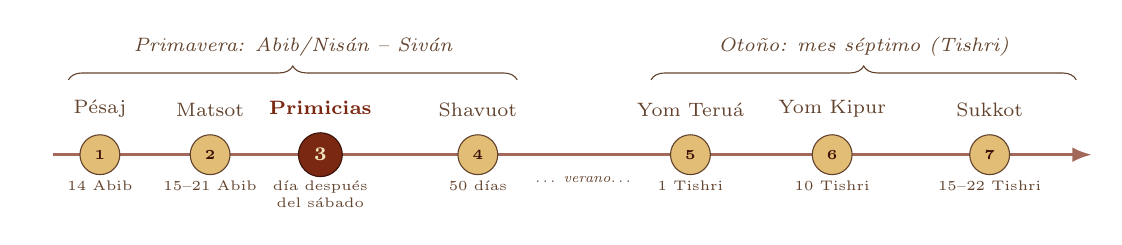
\begin{tikzpicture}[x=1cm,y=1cm,font=\scriptsize]
\def\fiestaactual{3}
 \draw[line width=1.2pt,tierraroja!70,-{Latex[length=2.5mm]}] (0,0) -- (13.2,0);
 \draw[decorate,decoration={brace,amplitude=5pt},sepia] (0.2,0.95) -- (5.9,0.95) node[midway,above=5pt,font=\scriptsize\itshape]{Primavera: Abib/Nisán -- Siván};
 \draw[decorate,decoration={brace,amplitude=5pt},sepia] (7.6,0.95) -- (13.0,0.95) node[midway,above=5pt,font=\scriptsize\itshape]{Otoño: mes séptimo (Tishri)};
 \foreach \n/\x/\t/\d in {1/0.6/Pésaj/{14 Abib},2/2.0/Matsot/{15--21 Abib},3/3.4/Primicias/{día después del sábado},4/5.4/Shavuot/{50 días},5/8.1/Yom Teruá/{1 Tishri},6/9.9/Yom Kipur/{10 Tishri},7/11.9/Sukkot/{15--22 Tishri}}{
   \ifnum\n=\fiestaactual
     \node[circle,fill=tierraroja,draw=caferojizo,minimum size=5.5mm,text=papiro,font=\scriptsize\bfseries] at (\x,0) {\n};
     \node[above=3pt,font=\scriptsize\bfseries,text=tierraroja] at (\x,0.28) {\t};
   \else
     \node[circle,fill=mostaza!70,draw=sepia,minimum size=4.5mm,text=caferojizo,font=\tiny\bfseries] at (\x,0) {\n};
     \node[above=3pt,text=sepia] at (\x,0.25) {\t};
   \fi
   \node[below=6pt,text width=1.6cm,align=center,font=\tiny,text=sepia] at (\x,0) {\d};}
 \node[font=\tiny\itshape,text=sepia] at (6.75,-0.32) {\ldots\ verano\ldots};
\end{tikzpicture}}\par\medskip
\small\RaggedRight La tercera ``estación'' de la primavera, \destacar{bisagra} entre los Ázimos (por la fecha) y Shavuot (por la cuenta y la estructura literaria).
\end{frame}


% ------------------------------------------------------------------
\section{El texto}

\begin{frame}{Texto ancla: Lv 23:9--11}
\fotolado{panel_levitico23_10.jpg}{Elaboración propia: Lv 23:10 en texto hebreo consonántico (BHS).}
\begin{columns}[c,onlytextwidth]
\begin{column}{0.57\textwidth}
\begin{cita}Y habló \SENOR{} a Moisés, diciendo: Habla a los hijos de Israel y diles: Cuando hayáis entrado en la tierra que yo os doy, y seguéis su mies, traeréis al sacerdote una gavilla por primicia de los primeros frutos de vuestra siega.\fuente{(Lv 23:9--10, RVR1960)}\end{cita}
\small\heb{עֹמֶר רֵאשִׁית קְצִירְכֶם} (\emph{ómer reshit qetsirjem}): la \destacar{gavilla, primera parte} de la siega. Ley dada para la tierra futura.
\end{column}
\begin{column}{0.41\textwidth}\end{column}
\end{columns}
\end{frame}

\begin{frame}{``Para que seáis aceptos''}
\fotolado{panel_levitico23_11.jpg}{Elaboración propia: Lv 23:11 en texto hebreo consonántico (BHS).}
\begin{columns}[c,onlytextwidth]
\begin{column}{0.57\textwidth}
\begin{cita}Y el sacerdote mecerá la gavilla delante de \SENOR, para que seáis aceptos; el día siguiente del día de reposo la mecerá.\fuente{(Lv 23:11, RVR1960)}\end{cita}
\small
\begin{itemize}
\item \heb{וְהֵנִיף} (\emph{heníf}): ``mecerá''; la gavilla es \emph{tenufá}.
\item \heb{לִרְצֹנְכֶם} (\emph{lirtsonjem}): quien queda aceptado es \destacar{el pueblo}.
\item \heb{מִמָּחֳרַת הַשַּׁבָּת}: una fecha \destacar{relativa}, sin número de día.
\end{itemize}
\end{column}
\begin{column}{0.41\textwidth}\end{column}
\end{columns}
\end{frame}

\begin{frame}{Los elementos del rito (Lv 23:9--14)}
\scriptsize\renewcommand{\arraystretch}{1.12}
\begin{tabular}{@{}L{2.2cm}L{3.3cm}L{6.4cm}@{}}
\toprule
\textbf{Elemento} & \textbf{Hebreo} & \textbf{Sentido} \\ \midrule
Condición & \heb{כִּי־תָבֹאוּ אֶל־הָאָרֶץ} & ``cuando hayáis entrado en la tierra'' (v. 10) \\
Objeto & \heb{עֹמֶר רֵאשִׁית} & la gavilla, primicia; de cebada (Éx 9:31) \\
Gesto & \heb{וְהֵנִיף} & ``mecerá'' delante del \SENOR{} (v. 11) \\
Holocausto & \heb{כֶּבֶשׂ תָּמִים בֶּן־שְׁנָתוֹ} & cordero de un año sin defecto (v. 12) \\
\emph{Minjá} y libación & \heb{שְׁנֵי עֶשְׂרֹנִים סֹלֶת} & dos décimas de flor de harina con aceite; un cuarto de hin de vino (v. 13) \\
Prohibición & \heb{וְלֶחֶם וְקָלִי וְכַרְמֶל} & ni pan, ni grano tostado, ni espiga fresca antes del rito (v. 14) \\
Vigencia & \heb{חֻקַּת עוֹלָם} & ``estatuto perpetuo\ldots{} dondequiera que habitéis'' (v. 14) \\
\bottomrule
\end{tabular}\par\medskip
\small\RaggedRight Sin \emph{mikrá kódesh} y sin prohibición de trabajo; la serie lo describe como ceremonia \destacar{sin ser un día de guardar}.
\end{frame}

\begin{frame}{La cuenta nace del Ómer}
\centering\heb{וּסְפַרְתֶּם לָכֶם מִמָּחֳרַת הַשַּׁבָּת} \foreignlanguage{spanish}{[\ldots]} \heb{שֶׁבַע שַׁבָּתוֹת תְּמִימֹת}
\begin{cita}Y contaréis desde el día que sigue al día de reposo, desde el día en que ofrecisteis la gavilla de la ofrenda mecida; siete semanas cumplidas serán. Hasta el día siguiente del séptimo día de reposo contaréis cincuenta días; entonces ofreceréis el nuevo grano a \SENOR.\fuente{(Lv 23:15--16, RVR1960)}\end{cita}
\small\RaggedRight
\begin{itemize}
\item \emph{usfartem}, ``y contaréis'': origen de la \emph{sefirá} posterior.
\item \emph{mimojorat hashabat} tres veces (vv. 11, 15, 16): define \destacar{a la vez} el Ómer y Pentecostés.
\end{itemize}
\end{frame}

\begin{frame}{Tabla sinóptica de las primicias}
\scriptsize\renewcommand{\arraystretch}{1.08}
\begin{tabular}{@{}L{2.0cm}L{4.6cm}L{5.3cm}@{}}
\toprule
\textbf{Texto} & \textbf{Qué ordena} & \textbf{Qué añade} \\ \midrule
Éx 23:16, 19 & ``las primicias de los primeros frutos'' a la casa de Dios & une \emph{reshit} y \emph{bikurim} \\
Éx 34:22, 26 & ``fiesta de las semanas'' & Shavuot, trigo \\
Lv 2:12, 14 & espigas verdes tostadas & procedimiento de la \emph{minjá} de primicias \\
Lv 23:9--14 & la gavilla mecida & fecha relativa; ``para que seáis aceptos'' \\
Lv 23:15--21 & siete semanas; dos panes con levadura & el Ómer abre, Shavuot cierra \\
Nm 15:20--21 & la primera masa & base de Ro 11:16 \\
Nm 18:12--13 & \emph{reshit} y \emph{bikurim} para los sacerdotes & los dos términos juntos \\
Nm 28:26 & ``el día de las primicias'' & Nm 28--29 \destacar{no} incluye el Ómer \\
Dt 16:9 & ``desde que comenzare a meterse la hoz'' & sin mención del ``sábado'' \\
Dt 26:1--11 & la canasta y la confesión & memoria del éxodo y de la tierra \\
\bottomrule
\end{tabular}
\end{frame}

\begin{frame}{El Ómer no es la canasta de Dt 26}
\begin{columns}[t,onlytextwidth]
\begin{column}{0.50\textwidth}
\centering\heb{אֲרַמִּי אֹבֵד אָבִי}
\begin{cita}Un arameo a punto de perecer fue mi padre, el cual descendió a Egipto\ldots{} Y ahora, he aquí he traído las primicias del fruto de la tierra que me diste, oh \SENOR.\fuente{(Dt 26:5, 10, RVR1960)}\end{cita}
\scriptsize\RaggedRight El fruto es la \destacar{última línea de un relato} que empieza en Egipto.
\end{column}
\begin{column}{0.48\textwidth}\small\RaggedRight
\begin{itemize}
\item Dt 26: \destacar{familiar}, sin fecha, con confesión; entre Shavuot y Sukkot según la Misná (Bikurim 1:3).
\item Lv 23: \destacar{nacional}, una gavilla, fecha precisa, sin palabras prescritas.
\end{itemize}
\precision{``arameo a punto de perecer'' = Jacob (ibn Ezra, Rashbam; Tigay, 1996); el Targum Onqelos y la Hagadá leen ``Labán el arameo quiso destruir a mi padre''.}
\end{column}
\end{columns}
\end{frame}

% ------------------------------------------------------------------
\section{Historia}

\begin{frame}{La cebada de Abib}
\begin{columns}[t,onlytextwidth]
\begin{column}{0.54\textwidth}
\centering\heb{כִּי הַשְּׂעֹרָה אָבִיב וְהַפִּשְׁתָּה גִּבְעֹל}
\begin{cita}El lino, pues, y la cebada fueron destrozados, porque la cebada estaba ya espigada, y el lino en caña.\fuente{(Éx 9:31, RVR1960)}\end{cita}
\begin{cita}\ldots{}y llegaron a Belén al comienzo de la siega de la cebada.\fuente{(Rut 1:22, RVR1960)}\end{cita}
\end{column}
\begin{column}{0.44\textwidth}\small\RaggedRight
\begin{itemize}
\item \emph{Abib}: cebada en espiga; \heb{חֹדֶשׁ הָאָבִיב}, ``mes de la espiga'' (Éx 13:4).
\item Cebada en Abib, trigo siete semanas después: la cuenta coincide con \destacar{la siega real}.
\item Calendario de Gézer (s. \textsc{x} a.\,e.\,c.): \heb{ירח קצר שערם}, ``mes de la siega de la cebada''.
\end{itemize}
\end{column}
\end{columns}
\end{frame}

\begin{frame}{Gilgal: el primer fruto de la tierra}
\centering\heb{וַיֹּאכְלוּ מֵעֲבוּר הָאָרֶץ מִמָּחֳרַת הַפֶּסַח מַצּוֹת וְקָלוּי}
\begin{cita}Al otro día de la pascua comieron del fruto de la tierra, los panes sin levadura, y en el mismo día espigas nuevas tostadas. Y el maná cesó el día siguiente\ldots\fuente{(Jos 5:11--12, RVR1960)}\end{cita}
\small\RaggedRight
\begin{itemize}
\item \heb{וְקָלוּי} y \heb{בְּעֶצֶם הַיּוֹם הַזֶּה}: el vocabulario de Lv 23:14.
\item Del \destacar{pan dado} (maná, medido por \emph{ómer}) al \destacar{pan cosechado}.
\end{itemize}
\precision{\emph{mimojorat hapésaj} = 15 de Abib en Nm 33:3; la tradición rabínica lee aquí el 16. Pieza del debate textual.}
\end{frame}

\begin{frame}{El Segundo Templo}
\begin{columns}[t,onlytextwidth]
\begin{column}{0.48\textwidth}\small\RaggedRight
\begin{itemize}
\item \destacar{Josefo}: ``el segundo día de los panes sin levadura, que es el decimosexto'' se ofrecen las primicias de la cebada (\emph{Ant.} 3.250--251; paráfrasis).
\item \destacar{Filón}: ``fiesta dentro de la fiesta''; la nación ofrece por todo el género humano (\emph{Spec.} 2.162--163).
\item 2~Cr 31:5; Neh 10:35: las primicias como \destacar{señal de reforma}.
\end{itemize}
\end{column}
\begin{column}{0.50\textwidth}
\begin{tcolorbox}[colback=mostaza!12,colframe=mostaza!85!tierraroja,boxrule=0.6pt,arc=2pt,title={\scriptsize\bfseries Tradición: Misná Menajot 10:3},coltitle=caferojizo,colbacktitle=mostaza!30,fontupper=\scriptsize]
\RaggedRight Noche del 15 al 16: ``¿Se ha puesto el sol?'' ---¡Sí! ``¿Con esta hoz?'' ---¡Sí! ``¿En esta canasta?'' ---¡Sí! ``¿Siego?'' ---¡Siega! Tres veces, ``por causa de los boetusianos''.
\end{tcolorbox}
\precision{tradición rabínica posterior al Templo; conserva una práctica y una polémica.}
\end{column}
\end{columns}
\end{frame}

\begin{frame}{Línea de tiempo}
\centering
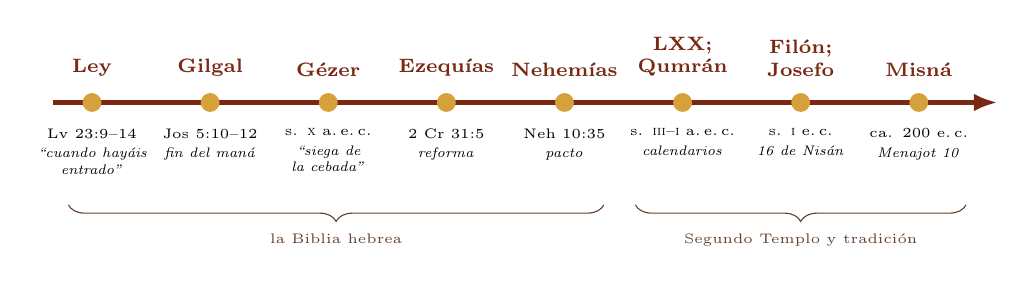
\begin{tikzpicture}[font=\scriptsize]
 \draw[line width=1.6pt,tierraroja,-{Latex[length=3mm]}] (0,0) -- (12.0,0);
 \foreach \x/\a/\b/\c in {0.5/{Ley}/{Lv 23:9--14}/{``cuando hayáis entrado''}, 2.0/{Gilgal}/{Jos 5:10--12}/{fin del maná}, 3.5/{Gézer}/{s. \textsc{x} a.\,e.\,c.}/{``siega de la cebada''}, 5.0/{Ezequías}/{2 Cr 31:5}/{reforma}, 6.5/{Nehemías}/{Neh 10:35}/{pacto}, 8.0/{LXX; Qumrán}/{s. \textsc{iii}--\textsc{i} a.\,e.\,c.}/{calendarios}, 9.5/{Filón; Josefo}/{s. \textsc{i} e.\,c.}/{16 de Nisán}, 11.0/{Misná}/{ca. 200 e.\,c.}/{Menajot 10}}{
   \fill[mostaza] (\x,0) circle (3.4pt);
   \node[above=6pt,font=\scriptsize\bfseries,text=tierraroja,text width=1.4cm,align=center] at (\x,0) {\a};
   \node[below=6pt,text width=1.4cm,align=center,font=\tiny] at (\x,0) {\b\\[1pt]\textit{\c}};}
 \draw[decorate,decoration={brace,amplitude=6pt,mirror},sepia] (0.2,-1.3) -- (7.0,-1.3) node[midway,below=7pt,font=\tiny,text=sepia] {la Biblia hebrea};
 \draw[decorate,decoration={brace,amplitude=6pt,mirror},sepia] (7.4,-1.3) -- (11.6,-1.3) node[midway,below=7pt,font=\tiny,text=sepia] {Segundo Templo y tradición};
\end{tikzpicture}\par\medskip
\precision{las fechas de la ley y de Josué dependen de la cronología del éxodo (serie: 1529 a.\,e.\,c.; 1~R 6:1: ca. 1446; fecha tardía: ca. 1260).}
\end{frame}

% ------------------------------------------------------------------
\section{Filología}

\begin{frame}{El campo semántico}
\centering
\begin{tikzpicture}[font=\scriptsize,
  t/.style={draw=tierraroja!70,line width=0.6pt,fill=papiro,fill opacity=0.9,text opacity=1,rounded corners=2pt,text width=2.75cm,align=center,inner sep=3pt}]
 \node[draw=tierraroja,line width=1pt,fill=mostaza!25,rounded corners=4pt,text width=2.7cm,align=center,inner sep=5pt] (c) at (0,0)
   {\small\bfseries\color{tierraroja} Lo primero pertenece a Dios\\[1pt]\normalfont\tiny\color{sepia}y consagra el resto (Ro 11:16)};
 \node[t] (r) at (-4.0,1.55) {\heb{רֵאשִׁית} \textbf{reshit}\\ lo primero y lo mejor\\ \textit{Lv 23:10; Pr 3:9}};
 \node[t] (b) at (0,2.15) {\heb{בִּכּוּרִים} \textbf{bikurim}\\ los primeros maduros\\ \textit{Éx 23:19; Nm 28:26}};
 \node[t] (k) at (4.0,1.55) {\heb{בְּכוֹר} \textbf{bejor}\\ el primogénito\\ \textit{Éx 4:22; 13:2}};
 \node[t] (o) at (-4.0,-1.55) {\heb{עֹמֶר} \textbf{ómer}\\ gavilla; décima de efa\\ \textit{Lv 23:10; Éx 16:36}};
 \node[t] (n) at (0,-2.15) {\heb{תְּנוּפָה} \textbf{tenufá}\\ lo mecido o elevado\\ \textit{Lv 23:11; Nm 8:11}};
 \node[t] (m) at (4.0,-1.55) {\heb{תְּרוּמָה} \textbf{terumá}\\ lo alzado y separado\\ \textit{Nm 15:20; 18:8}};
 \foreach \n in {r,b,k,o,n,m} \draw[sepia!80,line width=0.5pt] (c) -- (\n);
 \draw[mostaza!90!tierraroja,line width=0.8pt,dashed,{Latex[length=2mm]}-{Latex[length=2mm]}] (b.east) to[bend left=12] node[above,font=\tiny,text=sepia]{raíz \heb{בכר}} (k.north);
\end{tikzpicture}
\end{frame}

\begin{frame}{\emph{Reshit} y \emph{bikurim}}
\begin{columns}[t,onlytextwidth]
\begin{column}{0.49\textwidth}\small\RaggedRight
\textbf{\color{tierraroja}\heb{רֵאשִׁית} (\emph{reshit})}, de \emph{rosh}, ``cabeza'':
\begin{itemize}
\item tiempo: \heb{בְּרֵאשִׁית} (Gn 1:1); ``el principio de la sabiduría'' (Pr 1:7)
\item calidad: ``los ungüentos más preciosos'' (Am 6:6)
\item culto: \emph{reshit qetsirjem} (Lv 23:10); la primera masa (Nm 15:20)
\end{itemize}
\scriptsize LXX: \grc{ἀπαρχή}.
\end{column}
\begin{column}{0.49\textwidth}\small\RaggedRight
\textbf{\color{tierraroja}\heb{בִּכּוּרִים} (\emph{bikurim})}, raíz \heb{בכר}, ``madurar primero'':
\begin{itemize}
\item \emph{bikurá}: higo temprano (Os 9:10)
\item \emph{bejor}: ``Israel es mi hijo, mi primogénito'' (Éx 4:22)
\item \heb{רֵאשִׁית בִּכּוּרֵי אַדְמָתְךָ} (Éx 23:19)
\end{itemize}
\scriptsize LXX: \grc{πρωτογενήματα}.
\end{column}
\end{columns}\medskip
\small\RaggedRight \emph{Reshit} mira a la \destacar{posición}; \emph{bikurim}, a la \destacar{maduración}. La raíz de \emph{bikurim} une el campo y la familia.
\end{frame}

\begin{frame}{\emph{Tenufá}, \emph{terumá} y \emph{lirtsonjem}}
\begin{columns}[t,onlytextwidth]
\begin{column}{0.50\textwidth}\small\RaggedRight
\begin{itemize}
\item \heb{תְּנוּפָה} (\emph{tenufá}), de \heb{נוף}: ``mecer, blandir''. Rabinos: adelante y atrás, arriba y abajo (Menajot 5:6). \destacar{Milgrom (1991): ``elevación''}, gesto de dedicación (Nm 8:11: los levitas como \emph{tenufá}).
\item \heb{תְּרוּמָה} (\emph{terumá}), de \heb{רוּם}: lo ``alzado'' y separado (Nm 15:20; 18:8).
\end{itemize}
\end{column}
\begin{column}{0.48\textwidth}\small\RaggedRight
\heb{לִרְצֹנְכֶם}, ``para vuestra aceptación'' (Lv 23:11):
\begin{itemize}
\item LXX \grc{δεκτὸν ὑμῖν}
\item Is 61:2 \heb{שְׁנַת־רָצוֹן} $\rightarrow$ Lc 4:19 \grc{ἐνιαυτὸν κυρίου δεκτόν}
\item Is 49:8 $\rightarrow$ 2~Co 6:2 \grc{καιρῷ δεκτῷ}
\end{itemize}
\end{column}
\end{columns}
\end{frame}

\begin{frame}{De la gavilla a Pablo}
\centering
\begin{tikzpicture}[font=\scriptsize,
  b/.style={draw=tierraroja,line width=0.8pt,fill=papiro,fill opacity=0.9,text opacity=1,rounded corners=3pt,text width=2.45cm,align=center,inner sep=4pt,minimum height=2.3cm}]
 \node[b] (h) at (0,0) {\textbf{\color{tierraroja}Hebreo}\\ Lv 23:10\\[3pt]\heb{עֹמֶר רֵאשִׁית}\\[2pt]``gavilla, primicia''};
 \node[b] (g) at (3.15,0) {\textbf{\color{tierraroja}LXX}\\ Lv 23:10\\[3pt]\grc{δράγμα ἀπαρχήν}\\[2pt]``gavilla, primicia''};
 \node[b] (p) at (6.3,0) {\textbf{\color{tierraroja}Pablo}\\ 1 Co 15:20\\[3pt]\grc{ἀπαρχὴ τῶν κεκοιμημένων}\\[2pt]``primicia de los que han dormido''};
 \node[b] (e) at (9.45,0) {\textbf{\color{tierraroja}RVR1960}\\[3pt]``primicias de los que durmieron es hecho''};
 \foreach \a/\b in {h/g,g/p,p/e} \draw[-{Latex[length=2.5mm]},line width=1.2pt,mostaza] (\a) -- (\b);
\end{tikzpicture}\par\medskip
{\small\itshape\color{sepia} La gavilla que abría la siega se convierte en el nombre de Cristo resucitado, que abre la resurrección.}\par\medskip
\scriptsize\RaggedRight \grc{ἀπαρχή} en el NT (9 veces en SBLGNT y NA28; 8 en Westcott-Hort): 1~Co 15:20, 23; 16:15; Ro 8:23; 11:16; 16:5; 2~Ts 2:13 (NA28); Stg 1:18; Ap 14:4. \grc{πρωτότοκος}: Col 1:18; Ro 8:29; He 12:23.
\end{frame}

% ------------------------------------------------------------------
\section{Textual}

\begin{frame}{¿Qué ``sábado''? Tres lecturas}
\scriptsize\renewcommand{\arraystretch}{1.12}
\begin{tabular}{@{}L{2.2cm}L{2.4cm}L{1.8cm}L{1.9cm}L{2.9cm}@{}}
\toprule
\textbf{Grupo} & \textbf{``Sábado''} & \textbf{Ómer} & \textbf{Shavuot} & \textbf{Testimonios} \\ \midrule
Fariseos, rabinos & 15 Nisán (día festivo) & 16 Nisán & 6 Siván & LXX; Onqelos; Filón; Josefo; Misná \\
Saduceos, boetusianos, caraítas & sábado semanal dentro de los Ázimos & domingo, 16--22 & siempre domingo & Menajot 10:3 (como adversarios); caraítas; samaritanos \\
Qumrán, Jubileos & sábado semanal después de los Ázimos & domingo 26/I & domingo 15/III & 11Q19 18--19; Jub 6 \\
\bottomrule
\end{tabular}\par\medskip
\small\RaggedRight La definición del ``sábado'' de Lv 23:11 \destacar{decide también Pentecostés} (23:16).
\end{frame}

\begin{frame}{El mes de Abib y las tres fechas}
\centering
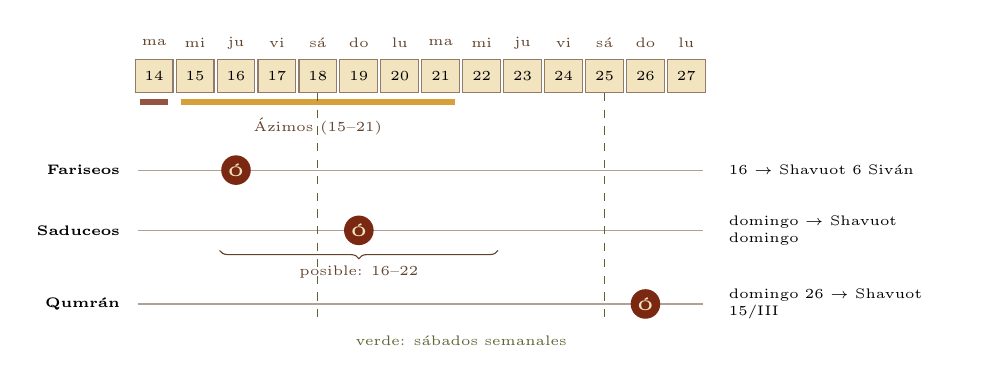
\begin{tikzpicture}[x=0.52cm,y=0.85cm,font=\tiny]
 \foreach \d [count=\i from 0] in {14,15,16,17,18,19,20,21,22,23,24,25,26,27}{
   \node[draw=sepia!70,fill=papiro,minimum width=0.48cm,minimum height=0.42cm,inner sep=0pt] at (\i,0) {\d};}
 \foreach \w [count=\i from 0] in {ma,mi,ju,vi,sá,do,lu,ma,mi,ju,vi,sá,do,lu}{\node[text=sepia] at (\i,0.5) {\w};}
 \fill[tierraroja!80] (-0.35,-0.42) rectangle (0.35,-0.34);
 \fill[mostaza] (0.65,-0.42) rectangle (7.35,-0.34);
 \node[text=sepia] at (4,-0.75) {Ázimos (15--21)};
 \node[anchor=east,align=right] at (-0.6,-1.4) {\textbf{Fariseos}};
 \draw[sepia!50] (-0.4,-1.4) -- (13.4,-1.4);
 \node[circle,fill=tierraroja,text=papiro,inner sep=1.2pt,font=\tiny\bfseries] at (2,-1.4) {Ó};
 \node[anchor=west,text width=2.9cm] at (13.8,-1.4) {16 $\rightarrow$ Shavuot 6 Siván};
 \node[anchor=east,align=right] at (-0.6,-2.3) {\textbf{Saduceos}};
 \draw[sepia!50] (-0.4,-2.3) -- (13.4,-2.3);
 \draw[decorate,decoration={brace,amplitude=3pt,mirror},sepia] (1.6,-2.6) -- (8.4,-2.6) node[midway,below=2pt]{posible: 16--22};
 \node[circle,fill=tierraroja,text=papiro,inner sep=1.2pt,font=\tiny\bfseries] at (5,-2.3) {Ó};
 \node[anchor=west,text width=2.9cm] at (13.8,-2.3) {domingo $\rightarrow$ Shavuot domingo};
 \node[anchor=east,align=right] at (-0.6,-3.4) {\textbf{Qumrán}};
 \draw[sepia!50] (-0.4,-3.4) -- (13.4,-3.4);
 \node[circle,fill=tierraroja,text=papiro,inner sep=1.2pt,font=\tiny\bfseries] at (12,-3.4) {Ó};
 \node[anchor=west,text width=2.9cm] at (13.8,-3.4) {domingo 26 $\rightarrow$ Shavuot 15/III};
 \foreach \s in {4,11}{\draw[oliva,dashed] (\s,-0.25) -- (\s,-3.7);}
 \node[text=oliva] at (7.5,-3.95) {verde: sábados semanales};
\end{tikzpicture}\par\smallskip
\precision{año ilustrativo con el 15 en miércoles (como siempre en Qumrán); en el calendario fariseo el 16 cae en cualquier día.}
\end{frame}

\begin{frame}{Los argumentos del texto}
\begin{columns}[t,onlytextwidth]
\begin{column}{0.33\textwidth}\scriptsize\RaggedRight
\textbf{\color{tierraroja}Sábado semanal}
\begin{itemize}
\item \emph{shabat} sin calificativo = séptimo día (v. 3)
\item ``siete \emph{shabatot}'', ``séptimo \emph{shabat}'' (vv. 15--16)
\end{itemize}
\end{column}
\begin{column}{0.33\textwidth}\scriptsize\RaggedRight
\textbf{\color{tierraroja}Día festivo (15)}
\begin{itemize}
\item días festivos llamados \emph{shabatón} (vv. 24, 39) y Kipur \emph{shabat shabatón} (v. 32)
\item \emph{shabat} = semana (Lv 25:8; Dt 16:9)
\item fecha fija, como las demás
\end{itemize}
\end{column}
\begin{column}{0.32\textwidth}\scriptsize\RaggedRight
\textbf{\color{tierraroja}Qumrán}
\begin{itemize}
\item la gavilla no interrumpe la fiesta
\item calendario de 364 días: fecha y día de la semana fijos (VanderKam, 1998)
\end{itemize}
\end{column}
\end{columns}\medskip
\begin{tcolorbox}[colback=mostaza!12,colframe=mostaza!85!tierraroja,boxrule=0.6pt,arc=2pt,title={\scriptsize\bfseries Precisión textual: la LXX},coltitle=caferojizo,colbacktitle=mostaza!30,fontupper=\scriptsize]
\RaggedRight Lv 23:11 LXX: \grc{τῇ ἐπαύριον τῆς πρώτης}, ``el día siguiente del \emph{primero}'' (lectura farisea); Lv 23:15: \grc{ἀπὸ τῆς ἐπαύριον τῶν σαββάτων}, literal. El texto aislado no zanja la cuestión (Wenham, 1979; Levine, 1989; Milgrom, 2001).
\end{tcolorbox}
\end{frame}

\begin{frame}{Variantes en el Nuevo Testamento}
\scriptsize\renewcommand{\arraystretch}{1.12}
\begin{tabular}{@{}L{1.4cm}L{4.9cm}L{5.6cm}@{}}
\toprule
\textbf{Texto} & \textbf{Lecturas} & \textbf{Qué cambia} \\ \midrule
2 Ts 2:13 & \grc{ἀπαρχήν} (B, 33, Vulgata; NA28) / \grc{ἀπ᾽ ἀρχῆς} ($\aleph$, D, mayoritario; RVR1960) & ``os escogió \emph{como primicias}'' o ``\emph{desde el principio}'' \\
Ro 16:5 & \grc{Ἀσίας} (NA28) / \grc{Ἀχαΐας} (RVR1960) & Epeneto, primicia ``de Asia'' o ``de Acaya'' \\
Lc 6:1 & \grc{ἐν σαββάτῳ δευτεροπρώτῳ} (bizantino) / omitido (NA28, RVR1960) & ¿primer sábado de la cuenta del ómer? (hipótesis desde Escalígero) \\
Mc 16:9 & final largo, ausente en $\aleph$ y B & el ``primer día'' está igual en Mc 16:2 \\
\bottomrule
\end{tabular}\par\medskip
\precision{en mayúsculas continuas, \grc{ΑΠΑΡΧΗΝ} y \grc{ΑΠΑΡΧΗΣ} difieren en una letra.}
\end{frame}

% ------------------------------------------------------------------
\section{Literatura}

\begin{frame}{Lv 23:9 abre una nueva unidad}
\centering
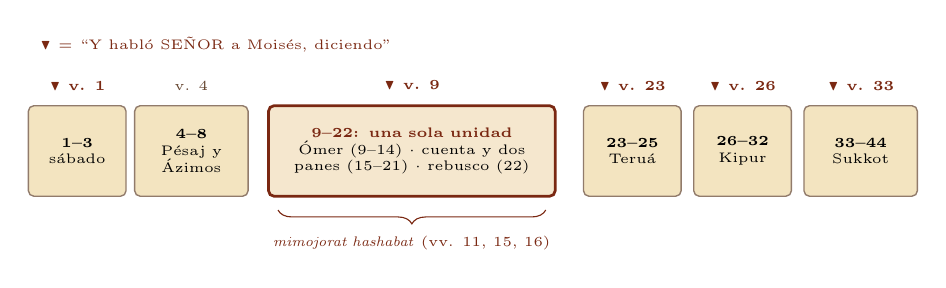
\begin{tikzpicture}[font=\tiny,
  u/.style={draw=sepia!70,line width=0.5pt,fill=papiro,rounded corners=2pt,minimum height=1.15cm,align=center,inner sep=2pt},
  h/.style={draw=tierraroja,line width=1pt,fill=mostaza!25,rounded corners=2pt,minimum height=1.15cm,align=center,inner sep=2pt}]
 \node[u,text width=1.1cm] (a) at (0,0) {\textbf{1--3}\\ sábado};
 \node[u,text width=1.3cm] (b) at (1.45,0) {\textbf{4--8}\\ Pésaj y Ázimos};
 \node[h,text width=3.5cm] (c) at (4.25,0) {\textbf{\color{tierraroja}9--22: una sola unidad}\\ Ómer (9--14) $\cdot$ cuenta y dos panes (15--21) $\cdot$ rebusco (22)};
 \node[u,text width=1.1cm] (d) at (7.05,0) {\textbf{23--25}\\ Teruá};
 \node[u,text width=1.1cm] (e) at (8.45,0) {\textbf{26--32}\\ Kipur};
 \node[u,text width=1.3cm] (f) at (9.95,0) {\textbf{33--44}\\ Sukkot};
 \foreach \n/\v in {a/1,c/9,d/23,e/26,f/33}{\node[text=tierraroja,font=\tiny\bfseries] at ([yshift=7pt]\n.north) {$\blacktriangledown$ v. \v};}
 \node[text=sepia] at ([yshift=7pt]b.north) {v. 4};
 \node[text=tierraroja,anchor=west] at (-0.6,1.35) {$\blacktriangledown$ = ``Y habló \SENOR{} a Moisés, diciendo''};
 \draw[decorate,decoration={brace,amplitude=5pt,mirror},tierraroja] (2.55,-0.75) -- (5.95,-0.75) node[midway,below=6pt,text=tierraroja]{\emph{mimojorat hashabat} (vv. 11, 15, 16)};
\end{tikzpicture}\par\bigskip
\small\RaggedRight Sin nueva introducción en el v. 15: el Ómer y Shavuot son \destacar{un mismo discurso}. Por la fecha, el Ómer está en los Ázimos; por la estructura, \destacar{mira a Pentecostés}. ``Cuando hayáis entrado'': ley de la tierra, como Lv 14:34; 19:23; 25:2.
\end{frame}

\begin{frame}{De la gavilla a los dos panes}
\centering
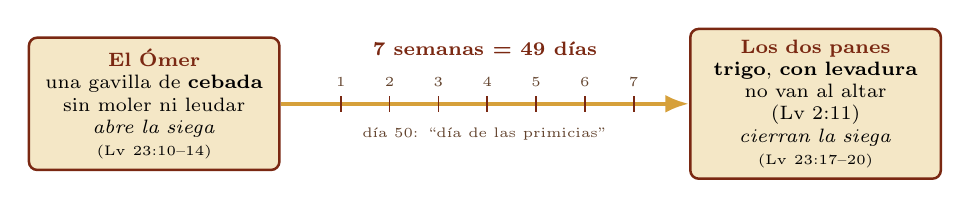
\begin{tikzpicture}[font=\scriptsize,
  g/.style={draw=tierraroja,line width=0.9pt,fill=papiro,fill opacity=0.9,text opacity=1,rounded corners=3pt,text width=2.9cm,align=center,inner sep=4pt}]
 \node[g] (o) at (0,0) {\textbf{\color{tierraroja}El Ómer}\\ una gavilla de \textbf{cebada}\\ sin moler ni leudar\\ \textit{abre la siega}\\ \tiny(Lv 23:10--14)};
 \node[g] (p) at (8.4,0) {\textbf{\color{tierraroja}Los dos panes}\\ \textbf{trigo}, \textbf{con levadura}\\ no van al altar (Lv 2:11)\\ \textit{cierran la siega}\\ \tiny(Lv 23:17--20)};
 \draw[line width=1.4pt,mostaza,-{Latex[length=3mm]}] (o.east) -- (p.west);
 \foreach \i in {1,...,7}{
   \pgfmathsetmacro{\xx}{1.75+\i*0.62}
   \draw[tierraroja,line width=0.6pt] (\xx,-0.1) -- (\xx,0.1);
   \node[font=\tiny,text=sepia] at (\xx,0.28) {\i};}
 \node[font=\scriptsize\bfseries,text=tierraroja] at (4.2,0.7) {7 semanas = 49 días};
 \node[font=\tiny,text=sepia] at (4.2,-0.38) {día 50: ``día de las primicias''};
\end{tikzpicture}\par\medskip
\small\RaggedRight Las dos ofrendas son \emph{tenufá} y ``primicias'' (\emph{reshit}, v. 10; \emph{bikurim}, vv. 17, 20). Del grano que brota al \destacar{pan de la casa}.\par\smallskip
\precision{lectura de la serie (lección 11): el Ómer = Cristo; los dos panes leudados = pueblos aún con pecado considerados para la redención.}\par\smallskip
\scriptsize\RaggedRight\destacar{Cuenta y jubileo}: \heb{וּסְפַרְתֶּם לָכֶם} (Lv 23:15) // \heb{וְסָפַרְתָּ לְךָ שֶׁבַע שַׁבְּתֹת שָׁנִים} (Lv 25:8): $7\times7$ días + 1 y $7\times7$ años + 1; la cuenta anual es miniatura del jubileo.
\end{frame}


\begin{frame}{``Lo primero para Dios''}
\centering
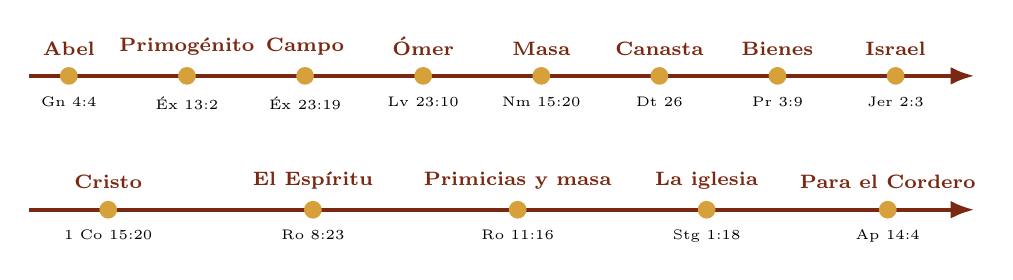
\begin{tikzpicture}[font=\scriptsize]
 \draw[line width=1.3pt,tierraroja,-{Latex[length=3mm]}] (0,0) -- (12.0,0);
 \foreach \x/\a/\b in {0.5/{Abel}/{Gn 4:4}, 2.0/{Primogénito}/{Éx 13:2}, 3.5/{Campo}/{Éx 23:19}, 5.0/{Ómer}/{Lv 23:10}, 6.5/{Masa}/{Nm 15:20}, 8.0/{Canasta}/{Dt 26}, 9.5/{Bienes}/{Pr 3:9}, 11.0/{Israel}/{Jer 2:3}}{
   \fill[mostaza] (\x,0) circle (3.2pt);
   \node[above=4pt,font=\scriptsize\bfseries,text=tierraroja] at (\x,0) {\a};
   \node[below=4pt,font=\tiny] at (\x,0) {\b};}
 \begin{scope}[yshift=-1.7cm]
 \draw[line width=1.3pt,tierraroja,-{Latex[length=3mm]}] (0,0) -- (12.0,0);
 \foreach \x/\a/\b in {1.0/{Cristo}/{1 Co 15:20}, 3.6/{El Espíritu}/{Ro 8:23}, 6.2/{Primicias y masa}/{Ro 11:16}, 8.6/{La iglesia}/{Stg 1:18}, 10.9/{Para el Cordero}/{Ap 14:4}}{
   \fill[mostaza] (\x,0) circle (3.2pt);
   \node[above=4pt,font=\scriptsize\bfseries,text=tierraroja] at (\x,0) {\a};
   \node[below=4pt,font=\tiny] at (\x,0) {\b};}
 \end{scope}
\end{tikzpicture}\par\medskip
\begin{cita}Si las primicias son santas, también lo es la masa restante\ldots\fuente{(Ro 11:16, RVR1960; cf. Nm 15:20--21)}\end{cita}
\small\RaggedRight La primicia no paga la cosecha, \destacar{la consagra}.
\end{frame}

% ------------------------------------------------------------------
\section{La serie}

\begin{frame}{Mención aparte: el Ómer}
\small\RaggedRight Sin ser un día de guardar, la presentación del Ómer fue una ofrenda de primicias con un profundo contenido espiritual. Representó al pueblo de Israel, que tras cruzar el mar Rojo quedó constituido como \destacar{la primicia de las naciones} rescatadas para Dios (Éx 19:5--6). En la era del Nuevo Pacto representa el sacrificio del Señor, que constituye al Hijo de Dios en \destacar{la primicia de los resucitados} para vida eterna.\par\medskip
\small\RaggedRight Tres partes: \destacar{memorial} (Israel primicia), \destacar{figura} (Cristo recibido a la diestra) y \destacar{vigencia} (rito cumplido).
\end{frame}

\begin{frame}{Israel, primicia: Jer 2:3}
\fotolado{panel_jeremias2_3.jpg}{Elaboración propia: Jer 2:3 en texto hebreo consonántico (BHS).}
\begin{columns}[c,onlytextwidth]
\begin{column}{0.57\textwidth}
\begin{cita}\ldots{}cuando andabas en pos de mí en el desierto, en tierra no sembrada. Santo era Israel a \SENOR, primicias de sus nuevos frutos.\fuente{(Jer 2:2--3, RVR1960)}\end{cita}
\scriptsize\RaggedRight
\begin{itemize}
\item \heb{רֵאשִׁית תְּבוּאָתֹה}: la palabra de Lv 23:10, \destacar{en el desierto}.
\item Éx 19:5--6: \emph{segulá} de ``toda la tierra''; Éx 4:22: ``mi primogénito''.
\item ``Todos los que le devoraban eran culpables'': quien come primicias profana (Lv 22:10).
\end{itemize}
\end{column}
\begin{column}{0.41\textwidth}\end{column}
\end{columns}
\end{frame}

\begin{frame}{Del 14 al 21 de Abib}
\centering
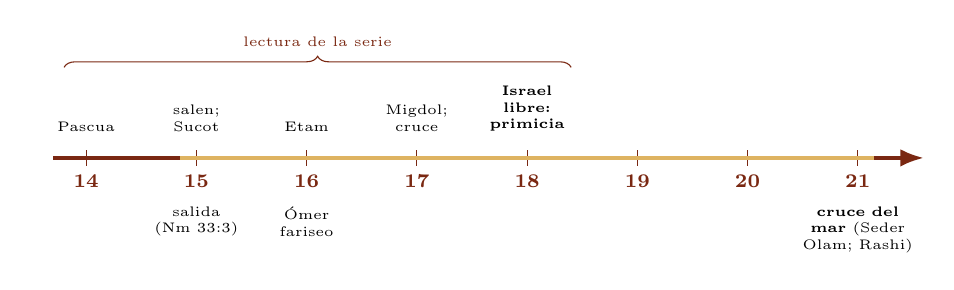
\begin{tikzpicture}[x=1.4cm,font=\tiny]
 \draw[line width=1.3pt,tierraroja,-{Latex[length=3mm]}] (-0.3,0) -- (7.6,0);
 \foreach \d [count=\i from 0] in {14,15,16,17,18,19,20,21}{\draw[tierraroja] (\i,-0.1) -- (\i,0.1); \node[font=\scriptsize\bfseries,text=tierraroja] at (\i,-0.3) {\d};}
 \foreach \i/\t in {0/{Pascua}, 1/{salen; Sucot}, 2/{Etam}, 3/{Migdol; cruce}, 4/{\textbf{Israel libre: primicia}}}{\node[above=6pt,text width=1.25cm,align=center] at (\i,0) {\t};}
 \draw[decorate,decoration={brace,amplitude=4pt},tierraroja] (-0.2,1.15) -- (4.4,1.15) node[midway,above=4pt,text=tierraroja]{lectura de la serie};
 \node[below=14pt,text width=1.3cm,align=center] at (1,0) {salida (Nm 33:3)};
 \node[below=14pt,text width=1.3cm,align=center] at (2,0) {Ómer fariseo};
 \node[below=14pt,text width=1.5cm,align=center] at (7,0) {\textbf{cruce del mar} (Seder Olam; Rashi)};
 \fill[mostaza!80] (0.85,0.03) rectangle (7.15,-0.03);
\end{tikzpicture}\par\medskip
\precision{la Biblia no fecha el cruce (Nm 33:5--8 no cuenta días por etapa). La tradición rabínica: 21 de Nisán (por eso se lee Éx 15). Éx 19:5--6 se dice ``en el mes tercero'' (Éx 19:1), y el Ómer es ley ``cuando hayáis entrado'': la lectura de la serie es \textbf{tipológica}; Jer 2:2--3 es su mejor apoyo.}
\end{frame}

\begin{frame}{Cristo recibido a la diestra}
\begin{columns}[t,onlytextwidth]
\begin{column}{0.53\textwidth}
\small\RaggedRight El Ómer de la ofrenda mecida representaba al Señor Jesús \destacar{en una nueva función}, tras ser recibido en el cielo a la diestra de Dios Padre.\par\smallskip
\scriptsize\RaggedRight Lectura \destacar{sacerdotal}: la gavilla era \emph{presentada} ``delante de \SENOR{}\ldots{} para que seáis aceptos''. Cristo entró ``para presentarse ahora por nosotros ante Dios'' (He 9:24).
\end{column}
\begin{column}{0.45\textwidth}
\small\RaggedRight Cumplido su objetivo, la ceremonia del Ómer \destacar{dejó de tener vigencia} para la Iglesia del Nuevo Pacto.\par\smallskip
\scriptsize\RaggedRight No era día de guardar y figuraba un hecho único. Pentecostés permanece (Hch 2:1).\par\smallskip
\precision{Lv 23:14 dice \emph{juqat olam}; la serie lo resuelve por cumplimiento. Autoría de Hebreos: discutida (Attridge, 1989; Lane, 1991).}
\end{column}
\end{columns}
\end{frame}

\begin{frame}{Mi lectura anterior: el rito}
\begin{columns}[t,onlytextwidth]
\begin{column}{0.50\textwidth}\small\RaggedRight
\textbf{\color{tierraroja}Lv 23:9--14 con glosas judías}
\begin{itemize}
\item ómer $\approx$ 3.500\,cm³ de cebada
\item ``el día posterior a Shabat'' = día posterior al primer día de Pésaj (lectura rabínica)
\item una sola gavilla, ``la gavilla de los primeros frutos'', mecida ``el día después del sábado'' con las ofrendas prescritas
\end{itemize}
\precision{el efa se estima entre unos 22 y 36 litros: el ómer va de $\approx$\,2,2 a 3,6 litros.}
\end{column}
\begin{column}{0.48\textwidth}\small\RaggedRight
\textbf{\color{tierraroja}El concepto de primicias}
\begin{itemize}
\item siempre \destacar{lo mejor y lo primero}
\item \destacar{santas} ante Dios: ``Conságrame todo primogénito'' (Éx 13:2); ``me darás el primogénito de tus hijos'' (Éx 22:29 [22:28])
\item presentadas \destacar{con alabanza} (Dt 26:1--11)
\end{itemize}
\end{column}
\end{columns}
\end{frame}

\begin{frame}{El diecisiete de Nisán}
\scriptsize\renewcommand{\arraystretch}{1.1}
\begin{tabular}{@{}L{2.5cm}L{3.6cm}L{5.8cm}@{}}
\toprule
\textbf{Hito} & \textbf{Mi cómputo} & \textbf{Precisión con el texto} \\ \midrule
Arca en el Ararat (Gn 8:4) & ``mes séptimo, a los diecisiete días'' desde Tishri = Nisán & el texto no nombra el mes; contado desde Nisán sería Tishri (Rosh haShaná 11b: R. Eliezer / R. Yehoshúa) \\
Cruce del mar (Éx 14) & salida el 15 + ``camino de tres días'' (Éx 3:18; 5:3) & los tres días son la petición al faraón; Éx 14 no fecha el cruce. serie: 17; rabinos: 21 \\
Primer fruto de la tierra (Jos 5:10--12) & ``cumplimiento histórico de Lv 23:9--13'' & ``al otro día de la pascua'' (15 o 16); el maná cesa ``el día siguiente'' (16 o 17) \\
Amán derrotado (Est 3--7) & decreto el 13 (Est 3:12); ayuno de tres días (4:16) & Ester no da la fecha; la tradición: el 16, con Mardoqueo enseñando las leyes del ómer (Meguilá 16a; verificar) \\
\bottomrule
\end{tabular}\par\medskip
\precision{cómputos tradicionales, no fechas explícitas: lectura tipológica mía, ``vida desde la muerte''.}
\end{frame}

\begin{frame}{Jesús, primicia de la cebada}
\begin{columns}[c,onlytextwidth]
\begin{column}{0.50\textwidth}\scriptsize\RaggedRight
\begin{itemize}
\item primogénito de María (Mt 1:23--25; Lc 2:7)
\item primogénito introducido por el Padre (He 1:6)
\item ``el primogénito de toda creación'' (Col 1:15)
\item ``el primogénito de los muertos'' (Ap 1:5)
\item ``primogénito entre muchos hermanos'' (Ro 8:29)
\item ``primicias de los que durmieron'' (1~Co 15:20, 23)
\item ``el principio de la creación de Dios'' (Ap 3:14)
\item ``que en todo tenga la preeminencia'' (Col 1:18)
\end{itemize}
\end{column}
\begin{column}{0.48\textwidth}
\begin{cita}Pero cada uno en su debido orden: Cristo, las primicias; luego los que son de Cristo, en su venida.\fuente{(1~Co 15:23, RVR1960)}\end{cita}
\scriptsize\RaggedRight Las dos raíces del campo: \emph{bejor} / \grc{πρωτότοκος} y \emph{reshit} / \grc{ἀρχή}, \grc{ἀπαρχή}.\par\smallskip
\precision{Mt 1:25 ``primogénito'': texto mayoritario (RVR1960); NA28 lo omite. Seguro en Lc 2:7.}
\end{column}
\end{columns}
\end{frame}

% ------------------------------------------------------------------
\section{Mesías}

\begin{frame}{``El primer día de la semana''}
\scriptsize\renewcommand{\arraystretch}{1.12}
\begin{tabular}{@{}L{3.2cm}L{2.4cm}L{2.6cm}L{3.6cm}@{}}
\toprule
\textbf{Cronología} & \textbf{Domingo} & \textbf{Ómer fariseo} & \textbf{Ómer saduceo} \\ \midrule
Juan: viernes 14 (Jn 19:14, 31) & 16 Nisán & domingo 16: \textbf{coincide} & domingo 16: \textbf{coincide} \\
Sinópticos: viernes 15 & 17 Nisán & sábado 16 & domingo 17: \textbf{coincide} \\
\textbf{\color{tierraroja}Serie (adoptada)}: miércoles 14; resurrección al cerrarse el sábado 17 & \textbf{domingo 18}: tumba vacía, Ómer & viernes 16 & \textbf{domingo 18: coincide}; presentación (Jn 20:17) \\
\bottomrule
\end{tabular}\par\medskip
\small\RaggedRight \grc{τῇ μιᾷ τῶν σαββάτων} (Mc 16:2; Jn 20:1): ``el uno de los sábados''; \grc{σάββατα} = semana, como \emph{shabatot} en Lv 23:15.\par\smallskip
\precision{cálculo propio. La tercera fila es la cronología de la serie: el domingo 18 de Abib, día del Ómer, coincide con el 18 en que la serie sitúa a Israel primicia. Las otras filas quedan como alternativas académicas.}
\end{frame}

\begin{frame}{Tres días y tres noches}
\begin{columns}[t,onlytextwidth]
\begin{column}{0.50\textwidth}
\begin{cita}\ldots{}así estará el Hijo del Hombre en el corazón de la tierra tres días y tres noches.\fuente{(Mt 12:40, RVR1960)}\end{cita}
\scriptsize\RaggedRight \textbf{Sombras del tercer día} (mi lectura): Gn 22:4; Éx 3:18; 5:3; 8:27 [8:23]; Est 4:15--17; Jon 1:17 [2:1]; Mt 16:21; Lc 24:44--46.\par\smallskip
\textbf{Mi cómputo anterior}: crucifixión el 14, resurrección el 17, sábado semanal en la semana de Pascua (Mc 16:1--6).\par\smallskip
\precision{alternativas académicas: viernes--domingo con cómputo inclusivo (Est 4:16; 5:1; Mt 27:63--64; Lc 24:21); Ómer fariseo el 16; calendario de los años 30/33 discutido; Mc 16:9 en el final largo.}
\end{column}
\begin{column}{0.48\textwidth}\scriptsize\RaggedRight
\begin{tcolorbox}[colback=papiro,colframe=tierraroja,boxrule=1pt,arc=3pt,title={\scriptsize\bfseries Lectura de la serie},coltitle=papiro,colbacktitle=tierraroja,fontupper=\scriptsize,left=3pt,right=3pt,top=2pt,bottom=2pt]
\RaggedRight
\textbf{14} miércoles: muerte y sepultura (Jn 19:31, 42).\par
\textbf{15} jueves: el ``gran día'', primer día de Ázimos (Jn 19:31).\par
\textbf{17} sábado: al cerrarse, ``tres días y tres noches'' (Mt 12:40); ``pasado el día de reposo'' (\grc{ὀψὲ σαββάτων}, Mt 28:1).\par
\textbf{18} domingo: ``el día siguiente del sábado'', tumba vacía (Mc 16:2); \destacar{día del Ómer}: Cristo se presenta como primicia (Jn 20:17; 1~Co 15:20). Coincide con el 18 de Abib de Israel primicia.
\end{tcolorbox}
\end{column}
\end{columns}
\end{frame}

\begin{frame}{Jn 20:17 y Mt 27:52--53}
\begin{columns}[t,onlytextwidth]
\begin{column}{0.49\textwidth}
\begin{cita}No me toques, porque aún no he subido a mi Padre\ldots\fuente{(Jn 20:17, RVR1960)}\end{cita}
\scriptsize\RaggedRight \grc{μή μου ἅπτου}: ``deja de retenerme'' (Brown, 1970; Keener, 2003). \destacar{Lectura tipológica} (IDU, 2011): como la gavilla, Cristo se presenta primero ante el Padre; después se deja tocar (Mt 28:9; Jn 20:27).
\end{column}
\begin{column}{0.49\textwidth}
\begin{cita}\ldots{}y muchos cuerpos de santos que habían dormido, se levantaron; y saliendo de los sepulcros, después de la resurrección de él\ldots\fuente{(Mt 27:52--53, RVR1960)}\end{cita}
\scriptsize\RaggedRight \grc{τῶν κεκοιμημένων ἁγίων}: el participio de 1~Co 15:20. Cristo va \destacar{primero}. Algunos ven aquí la ``gavilla'' (Chumney, 1994).
\end{column}
\end{columns}\medskip
\precision{Juan y Mateo no mencionan el Ómer; son ecos posibles.}
\end{frame}

\begin{frame}{1~Co 15:20 en uncial}
\fotolado{panel_1corintios15.jpg}{Elaboración propia: 1~Co 15:20 en escritura uncial (texto NA28).}
\begin{columns}[c,onlytextwidth]
\begin{column}{0.57\textwidth}
\begin{cita}Mas ahora Cristo ha resucitado de los muertos; primicias de los que durmieron es hecho.\fuente{(1~Co 15:20, RVR1960)}\end{cita}
\small\RaggedRight \grc{Νυνὶ δὲ Χριστὸς ἐγήγερται ἐκ νεκρῶν ἀπαρχὴ τῶν κεκοιμημένων.}\par\medskip
\scriptsize La primicia es la primera parte de \destacar{la misma} cosecha y garantiza el resto (Fee, 1987; Thiselton, 2000). La misma carta: ``nuestra pascua'' (5:7) y Pentecostés (16:8).
\end{column}
\begin{column}{0.41\textwidth}\end{column}
\end{columns}
\end{frame}

\begin{frame}{``Cada uno en su debido orden''}
\centering
\begin{tikzpicture}[font=\scriptsize,
  s/.style={draw=tierraroja,line width=0.9pt,fill=papiro,fill opacity=0.9,text opacity=1,rounded corners=3pt,text width=2.5cm,align=center,inner sep=4pt,minimum height=2.2cm},
  d/.style={draw=sepia!70,dashed,line width=0.6pt,fill=papiro,fill opacity=0.6,text opacity=1,rounded corners=3pt,text width=2.0cm,align=center,inner sep=3pt,minimum height=2.2cm,font=\tiny}]
 \node[s] (a) at (0,0) {\textbf{\color{tierraroja}\grc{ἀπαρχὴ Χριστός}}\\[2pt]``Cristo, las primicias''\\ (15:20, 23)\\[2pt]\textit{Primicias}};
 \node[d] (p) at (2.95,0) {\textit{entre ambas}\\ ``primicias del Espíritu'' (Ro 8:23)\\[2pt]\textit{Pentecostés}};
 \node[s] (b) at (5.9,0) {\textbf{\color{tierraroja}\grc{οἱ τοῦ Χριστοῦ}}\\[2pt]``en su venida'' (15:23); ``la final trompeta'' (15:52)\\[2pt]\textit{Trompetas}};
 \node[s] (c) at (8.95,0) {\textbf{\color{tierraroja}\grc{τὸ τέλος}}\\[2pt]``luego el fin'': el reino entregado al Padre (15:24--28)\\[2pt]\textit{Octavo día}};
 \draw[-{Latex[length=2.5mm]},line width=1.2pt,mostaza] (a) -- (p);
 \draw[-{Latex[length=2.5mm]},line width=1.2pt,mostaza] (p) -- (b);
 \draw[-{Latex[length=2.5mm]},line width=1.2pt,mostaza] (b) -- (c);
\end{tikzpicture}\par\medskip
\small\RaggedRight \grc{τάγμα} (v. 23): orden, formación. En cursiva: lectura de la serie.\par\smallskip
\precision{Pablo no nombra las fiestas: la correspondencia es tipológica. ¿Intervalo entre venida y fin? Premilenaristas y la serie (Ap 20) sí; Fee (1987) y Thiselton (2000), no necesariamente.}
\end{frame}

\begin{frame}{La iglesia, primicias}
\begin{columns}[t,onlytextwidth]
\begin{column}{0.50\textwidth}
\begin{cita}\ldots{}nosotros mismos, que tenemos las primicias del Espíritu\ldots{} esperando la adopción, la redención de nuestro cuerpo.\fuente{(Ro 8:23, RVR1960)}\end{cita}
\begin{cita}\ldots{}para que seamos primicias de sus criaturas.\fuente{(Stg 1:18, RVR1960)}\end{cita}
\end{column}
\begin{column}{0.48\textwidth}
\begin{cita}Estos fueron redimidos de entre los hombres como primicias para Dios y para el Cordero.\fuente{(Ap 14:4, RVR1960)}\end{cita}
\scriptsize\RaggedRight Después vienen \destacar{dos siegas} (Ap 14:14--20): la primicia precede a la cosecha. Cristo, \grc{ἀρχή, πρωτότοκος ἐκ τῶν νεκρῶν} (Col 1:18).\par\smallskip
\precision{Colosenses y 2~Ts: autoría discutida; el argumento se apoya en 1~Co y Romanos.}
\end{column}
\end{columns}
\end{frame}

% ------------------------------------------------------------------
\section{Tradición}

\begin{frame}{La cuenta del ómer y Shavuot}
\begin{columns}[t,onlytextwidth]
\begin{column}{0.50\textwidth}\small\RaggedRight
\textbf{\color{tierraroja}\heb{סְפִירַת הָעֹמֶר}} (\emph{sefirat haómer})
\begin{itemize}
\item cada noche desde el 16 de Nisán, con bendición: ``hoy es el día\ldots{} del ómer''
\item ¿precepto o memorial sin Templo? (Menajot 66a)
\item semiduelo (Yevamot 62b); \emph{Lag baÓmer}, día 33
\end{itemize}
\end{column}
\begin{column}{0.48\textwidth}\small\RaggedRight
\begin{itemize}
\item 6 de Siván: Shavuot como \destacar{fiesta de la Torá} (Shabat 86b: ¿6 o 7?)
\item caraítas y samaritanos: siempre domingo
\item cristianos: Pentecostés desde el domingo de Pascua
\item \emph{Yom haBikurim} hoy (Chumney, 1994)
\end{itemize}
\end{column}
\end{columns}\medskip
\precision{todo es tradición posterior a la Biblia y al Nuevo Testamento.}
\end{frame}

% ------------------------------------------------------------------
\section{Debate}

\begin{frame}{Cuatro debates abiertos}
\centering
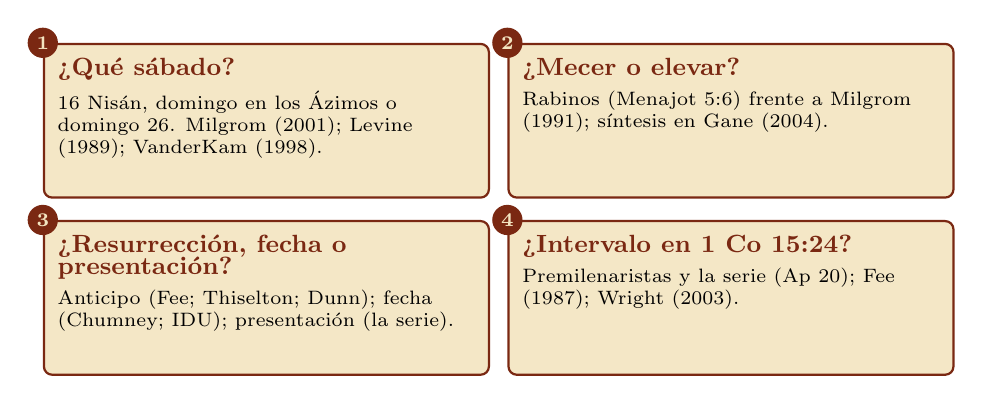
\begin{tikzpicture}
 \foreach \x/\y/\n/\t/\d in {0/0/1/{¿Qué sábado?}/{16 Nisán, domingo en los Ázimos o domingo 26. Milgrom (2001); Levine (1989); VanderKam (1998).}, 5.9/0/2/{¿Mecer o elevar?}/{Rabinos (Menajot 5:6) frente a Milgrom (1991); síntesis en Gane (2004).}, 0/-2.25/3/{¿Resurrección, fecha o presentación?}/{Anticipo (Fee; Thiselton; Dunn); fecha (Chumney; IDU); presentación (la serie).}, 5.9/-2.25/4/{¿Intervalo en 1 Co 15:24?}/{Premilenaristas y la serie (Ap 20); Fee (1987); Wright (2003).}}{
  \node[caja,anchor=north] (b\n) at (\x,\y) {\parbox[t][1.6cm][t]{5.3cm}{\RaggedRight
    {\small\textbf{\textcolor{tierraroja}{\t}}}\\[3pt]\scriptsize \d}};
  \node[circle,fill=tierraroja,text=papiro,font=\scriptsize\bfseries,inner sep=1.6pt] at (b\n.north west) {\n};}
\end{tikzpicture}\par\medskip
\small\RaggedRight La Escritura no da un número para el Ómer, y quienes quisieron obedecerla leyeron ese silencio de modos distintos.
\end{frame}

% ------------------------------------------------------------------
\section{Síntesis}

\begin{frame}{Definición}
\begin{tcolorbox}[colback=papiro,colframe=tierraroja,boxrule=1pt,arc=3pt,fontupper=\small]
\RaggedRight El \destacar{Ómer} es la primera gavilla de la siega, presentada ``delante de \SENOR'' el día siguiente del sábado de los Ázimos, ``para que seáis aceptos'' (Lv 23:10--11). Libera la cosecha nueva (23:14) y abre la cuenta hacia Pentecostés (23:15--16). Expresa la ley de toda la Escritura: \destacar{lo primero pertenece a Dios y consagra el resto} (Gn 4:4; Ro 11:16). Israel fue ``primicias de sus nuevos frutos'' (Jer 2:3); Cristo es ``primicias de los que durmieron'' (1~Co 15:20); la iglesia, ``primicias de sus criaturas'' (Stg 1:18). Cronología de la serie: resurrección al cerrarse el sábado 17; presentación como primicia el \destacar{18 de Abib}, el día siguiente del sábado.
\end{tcolorbox}
\centering\small\itshape ``Cristo, las primicias; luego los que son de Cristo, en su venida. Luego el fin'' (1~Co 15:23--24).
\end{frame}


% ------------------------------------------------------------------
\section{Reflexión}

\begin{frame}{Para la reflexión}
\small\RaggedRight
\begin{enumerate}
\item ¿Qué ``primera gavilla'' de su tiempo o sus bienes entrega antes de disponer del resto (Pr 3:9--10)?
\item ¿Qué cambia saber que su aceptación descansa en una primicia presentada por otro (Lv 23:11; He 9:24)?
\item ¿Qué rasgos de la ``juventud'' en el desierto conserva su comunidad (Jer 2:2--3)?
\item ¿Cómo enfrenta la muerte de un cercano sabiendo que la siega ya empezó con Cristo (1~Co 15:20, 23)?
\item ¿Cómo distinguir lo que el texto dice de lo que nuestra tradición decide (``el día siguiente del sábado'')?
\end{enumerate}
\end{frame}

% ------------------------------------------------------------------
\section{Glosario}

\begin{frame}{Glosario}
\scriptsize
\begin{columns}[t,onlytextwidth]
\begin{column}{0.49\textwidth}\RaggedRight
\textbf{Abib} (\heb{אָבִיב}): cebada en espiga; primer mes.\par
\textbf{Aparjé} (\grc{ἀπαρχή}): primicia (LXX; 1~Co 15:20).\par
\textbf{Bejor} (\heb{בְּכוֹר}): primogénito (Éx 4:22).\par
\textbf{Bikurim} (\heb{בִּכּוּרִים}): primeros maduros (Nm 28:26).\par
\textbf{Boetusianos}: contaban desde el domingo (Menajot 10:3).\par
\textbf{Drágma} (\grc{δράγμα}): gavilla (LXX Lv 23:10).\par
\textbf{Lirtsonjem} (\heb{לִרְצֹנְכֶם}): ``para que seáis aceptos''.\par
\textbf{Mimojorat hashabat} (\heb{מִמָּחֳרַת הַשַּׁבָּת}): ``el día siguiente del sábado''.
\end{column}
\begin{column}{0.49\textwidth}\RaggedRight
\textbf{Minjá} (\heb{מִנְחָה}): ofrenda vegetal (Lv 23:13).\par
\textbf{Ómer} (\heb{עֹמֶר}): gavilla; décima de efa (Éx 16:36).\par
\textbf{Prōtótokos} (\grc{πρωτότοκος}): primogénito (Col 1:18).\par
\textbf{Reshit} (\heb{רֵאשִׁית}): lo primero y lo mejor (Lv 23:10).\par
\textbf{Sefirat haómer} (\heb{סְפִירַת הָעֹמֶר}): cuenta rabínica de 49 días.\par
\textbf{Tenufá} (\heb{תְּנוּפָה}): ofrenda mecida o elevada.\par
\textbf{Terumá} (\heb{תְּרוּמָה}): lo alzado y separado (Nm 15:20).
\end{column}
\end{columns}
\end{frame}

% ------------------------------------------------------------------
\section{Referencias}

\begin{frame}{Referencias (1)}
\fontsize{6.2}{7.4}\selectfont
\begin{columns}[t,onlytextwidth]
\begin{column}{0.49\textwidth}
\refapa{Attridge, H.~W. (1989). \emph{The epistle to the Hebrews} (Hermeneia). Fortress.}
\refapa{Bauer, W., Danker, F.~W., Arndt, W.~F., \& Gingrich, F.~W. (2000). \emph{A Greek-English lexicon of the New Testament} (3.ª ed.). University of Chicago Press.}
\refapa{Brown, F., Driver, S.~R., \& Briggs, C.~A. (1906). \emph{A Hebrew and English lexicon of the Old Testament}. Clarendon.}
\refapa{Brown, R.~E. (1970). \emph{The Gospel according to John XIII--XXI} (AB 29A). Doubleday.}
\refapa{Chumney, E. (1994). \emph{The seven festivals of the Messiah}. Destiny Image.}
\refapa{Danby, H. (Trad.). (1933). \emph{The Mishnah}. Oxford University Press.}
\refapa{de Vaux, R. (1985). \emph{Instituciones del Antiguo Testamento} (4.ª ed.). Herder.}
\refapa{Dunn, J.~D.~G. (1998). \emph{The theology of Paul the apostle}. Eerdmans.}
\refapa{Edersheim, A. (1874). \emph{The Temple: Its ministry and services}. Religious Tract Society.}
\refapa{Elliger, K., \& Rudolph, W. (Eds.). (1997). \emph{Biblia Hebraica Stuttgartensia} (5.ª ed.). Deutsche Bibelgesellschaft.}
\refapa{Fee, G.~D. (1987). \emph{The first epistle to the Corinthians} (NICNT). Eerdmans.}
\refapa{Filón de Alejandría. (1937). \emph{De specialibus legibus} (F.~H. Colson, Trad.; LCL 320). Harvard University Press.}
\end{column}
\begin{column}{0.49\textwidth}
\refapa{Gane, R. (2004). \emph{Leviticus, Numbers} (NIVAC). Zondervan.}
\refapa{Hartley, J.~E. (1992). \emph{Leviticus} (WBC 4). Word.}
\refapa{Hays, R.~B. (1989). \emph{Echoes of Scripture in the letters of Paul}. Yale University Press.}
\refapa{Josefo, F. (1997). \emph{Antigüedades judías} (J. Vara Donado, Trad.). Akal.}
\refapa{Keener, C.~S. (2003). \emph{The Gospel of John}. Hendrickson.}
\refapa{Koehler, L., \& Baumgartner, W. (2001). \emph{The Hebrew and Aramaic lexicon of the Old Testament}. Brill.}
\end{column}
\end{columns}
\end{frame}

\begin{frame}{Referencias (2)}
\fontsize{6.2}{7.4}\selectfont
\begin{columns}[t,onlytextwidth]
\begin{column}{0.49\textwidth}
\refapa{Lane, W.~L. (1991). \emph{Hebrews} (WBC 47A--B). Word.}
\refapa{Levine, B.~A. (1989). \emph{Leviticus} (JPS Torah Commentary). Jewish Publication Society.}
\refapa{Milgrom, J. (1991). \emph{Leviticus 1--16} (AB 3). Doubleday.}
\refapa{Milgrom, J. (2001). \emph{Leviticus 23--27} (AB 3B). Doubleday.}
\refapa{Nestle, E., \& Aland, K. (Eds.). (2012). \emph{Novum Testamentum Graece} (28.ª ed.). Deutsche Bibelgesellschaft.}
\refapa{Rahlfs, A., \& Hanhart, R. (Eds.). (2006). \emph{Septuaginta}. Deutsche Bibelgesellschaft.}
\end{column}
\begin{column}{0.49\textwidth}
\refapa{Sefaria. (s.~f.). \emph{Misná y Talmud Menajot; Yevamot; Shabat; Seder Olam; Rashi}. https://www.sefaria.org}
\refapa{Thiselton, A.~C. (2000). \emph{The first epistle to the Corinthians} (NIGTC). Eerdmans.}
\refapa{Tigay, J.~H. (1996). \emph{Deuteronomy} (JPS Torah Commentary). Jewish Publication Society.}
\refapa{VanderKam, J.~C. (1998). \emph{Calendars in the Dead Sea Scrolls}. Routledge.}
\refapa{Wenham, G.~J. (1979). \emph{The book of Leviticus} (NICOT). Eerdmans.}
\refapa{Wright, N.~T. (2003). \emph{The resurrection of the Son of God}. Fortress.}
\refapa{Yadin, Y. (1983). \emph{The Temple Scroll} (3 vols.). Israel Exploration Society.}
\vspace{3pt}{\color{sepia}\textit{Nota sobre el texto.} Citas: Reina-Valera 1960 (\SENOR{} por ``Jehová''), cotejada en línea; hebreo BHS; griego NA28 y LXX Rahlfs-Hanhart. Misná, Talmud, targumes y Rashi, como tradición (Sefaria; Danby, 1933). Conteos: morfología WLC y SBLGNT del repositorio. Marco: la lectura de la serie y mi presentación \emph{Los Panes sin Levadura}. Paneles: elaboración propia.}
\end{column}
\end{columns}
\end{frame}


\end{document}
